\documentclass[1p]{elsarticle_modified}
%\bibliographystyle{elsarticle-num}

%\usepackage[colorlinks]{hyperref}
%\usepackage{abbrmath_seonhwa} %\Abb, \Ascr, \Acal ,\Abf, \Afrak
\usepackage{amsfonts}
\usepackage{amssymb}
\usepackage{amsmath}
\usepackage{amsthm}
\usepackage{scalefnt}
\usepackage{amsbsy}
\usepackage{kotex}
\usepackage{caption}
\usepackage{subfig}
\usepackage{color}
\usepackage{graphicx}
\usepackage{xcolor} %% white, black, red, green, blue, cyan, magenta, yellow
\usepackage{float}
\usepackage{setspace}
\usepackage{hyperref}

\usepackage{tikz}
\usetikzlibrary{arrows}

\usepackage{multirow}
\usepackage{array} % fixed length table
\usepackage{hhline}

%%%%%%%%%%%%%%%%%%%%%
\makeatletter
\renewcommand*\env@matrix[1][\arraystretch]{%
	\edef\arraystretch{#1}%
	\hskip -\arraycolsep
	\let\@ifnextchar\new@ifnextchar
	\array{*\c@MaxMatrixCols c}}
\makeatother %https://tex.stackexchange.com/questions/14071/how-can-i-increase-the-line-spacing-in-a-matrix
%%%%%%%%%%%%%%%

\usepackage[normalem]{ulem}

\newcommand{\msout}[1]{\ifmmode\text{\sout{\ensuremath{#1}}}\else\sout{#1}\fi}
%SOURCE: \msout is \stkout macro in https://tex.stackexchange.com/questions/20609/strikeout-in-math-mode

\newcommand{\cancel}[1]{
	\ifmmode
	{\color{red}\msout{#1}}
	\else
	{\color{red}\sout{#1}}
	\fi
}

\newcommand{\add}[1]{
	{\color{blue}\uwave{#1}}
}

\newcommand{\replace}[2]{
	\ifmmode
	{\color{red}\msout{#1}}{\color{blue}\uwave{#2}}
	\else
	{\color{red}\sout{#1}}{\color{blue}\uwave{#2}}
	\fi
}

\newcommand{\Sol}{\mathcal{S}} %segment
\newcommand{\D}{D} %diagram
\newcommand{\A}{\mathcal{A}} %arc


%%%%%%%%%%%%%%%%%%%%%%%%%%%%%5 test

\def\sl{\operatorname{\textup{SL}}(2,\Cbb)}
\def\psl{\operatorname{\textup{PSL}}(2,\Cbb)}
\def\quan{\mkern 1mu \triangleright \mkern 1mu}

\theoremstyle{definition}
\newtheorem{thm}{Theorem}[section]
\newtheorem{prop}[thm]{Proposition}
\newtheorem{lem}[thm]{Lemma}
\newtheorem{ques}[thm]{Question}
\newtheorem{cor}[thm]{Corollary}
\newtheorem{defn}[thm]{Definition}
\newtheorem{exam}[thm]{Example}
\newtheorem{rmk}[thm]{Remark}
\newtheorem{alg}[thm]{Algorithm}

\newcommand{\I}{\sqrt{-1}}
\begin{document}

%\begin{frontmatter}
%
%\title{Boundary parabolic representations of knots up to 8 crossings}
%
%%% Group authors per affiliation:
%\author{Yunhi Cho} 
%\address{Department of Mathematics, University of Seoul, Seoul, Korea}
%\ead{yhcho@uos.ac.kr}
%
%
%\author{Seonhwa Kim} %\fnref{s_kim}}
%\address{Center for Geometry and Physics, Institute for Basic Science, Pohang, 37673, Korea}
%\ead{ryeona17@ibs.re.kr}
%
%\author{Hyuk Kim}
%\address{Department of Mathematical Sciences, Seoul National University, Seoul 08826, Korea}
%\ead{hyukkim@snu.ac.kr}
%
%\author{Seokbeom Yoon}
%\address{Department of Mathematical Sciences, Seoul National University, Seoul, 08826,  Korea}
%\ead{sbyoon15@snu.ac.kr}
%
%\begin{abstract}
%We find all boundary parabolic representation of knots up to 8 crossings.
%
%\end{abstract}
%\begin{keyword}
%    \MSC[2010] 57M25 
%\end{keyword}
%
%\end{frontmatter}

%\linenumbers
%\tableofcontents
%
\newcommand\colored[1]{\textcolor{white}{\rule[-0.35ex]{0.8em}{1.4ex}}\kern-0.8em\color{red} #1}%
%\newcommand\colored[1]{\textcolor{white}{ #1}\kern-2.17ex	\textcolor{white}{ #1}\kern-1.81ex	\textcolor{white}{ #1}\kern-2.15ex\color{red}#1	}

{\Large $\underline{11a_{176}~(K11a_{176})}$}

\setlength{\tabcolsep}{10pt}
\renewcommand{\arraystretch}{1.6}
\vspace{1cm}\begin{tabular}{m{100pt}>{\centering\arraybackslash}m{274pt}}
\multirow{5}{120pt}{
	\centering
	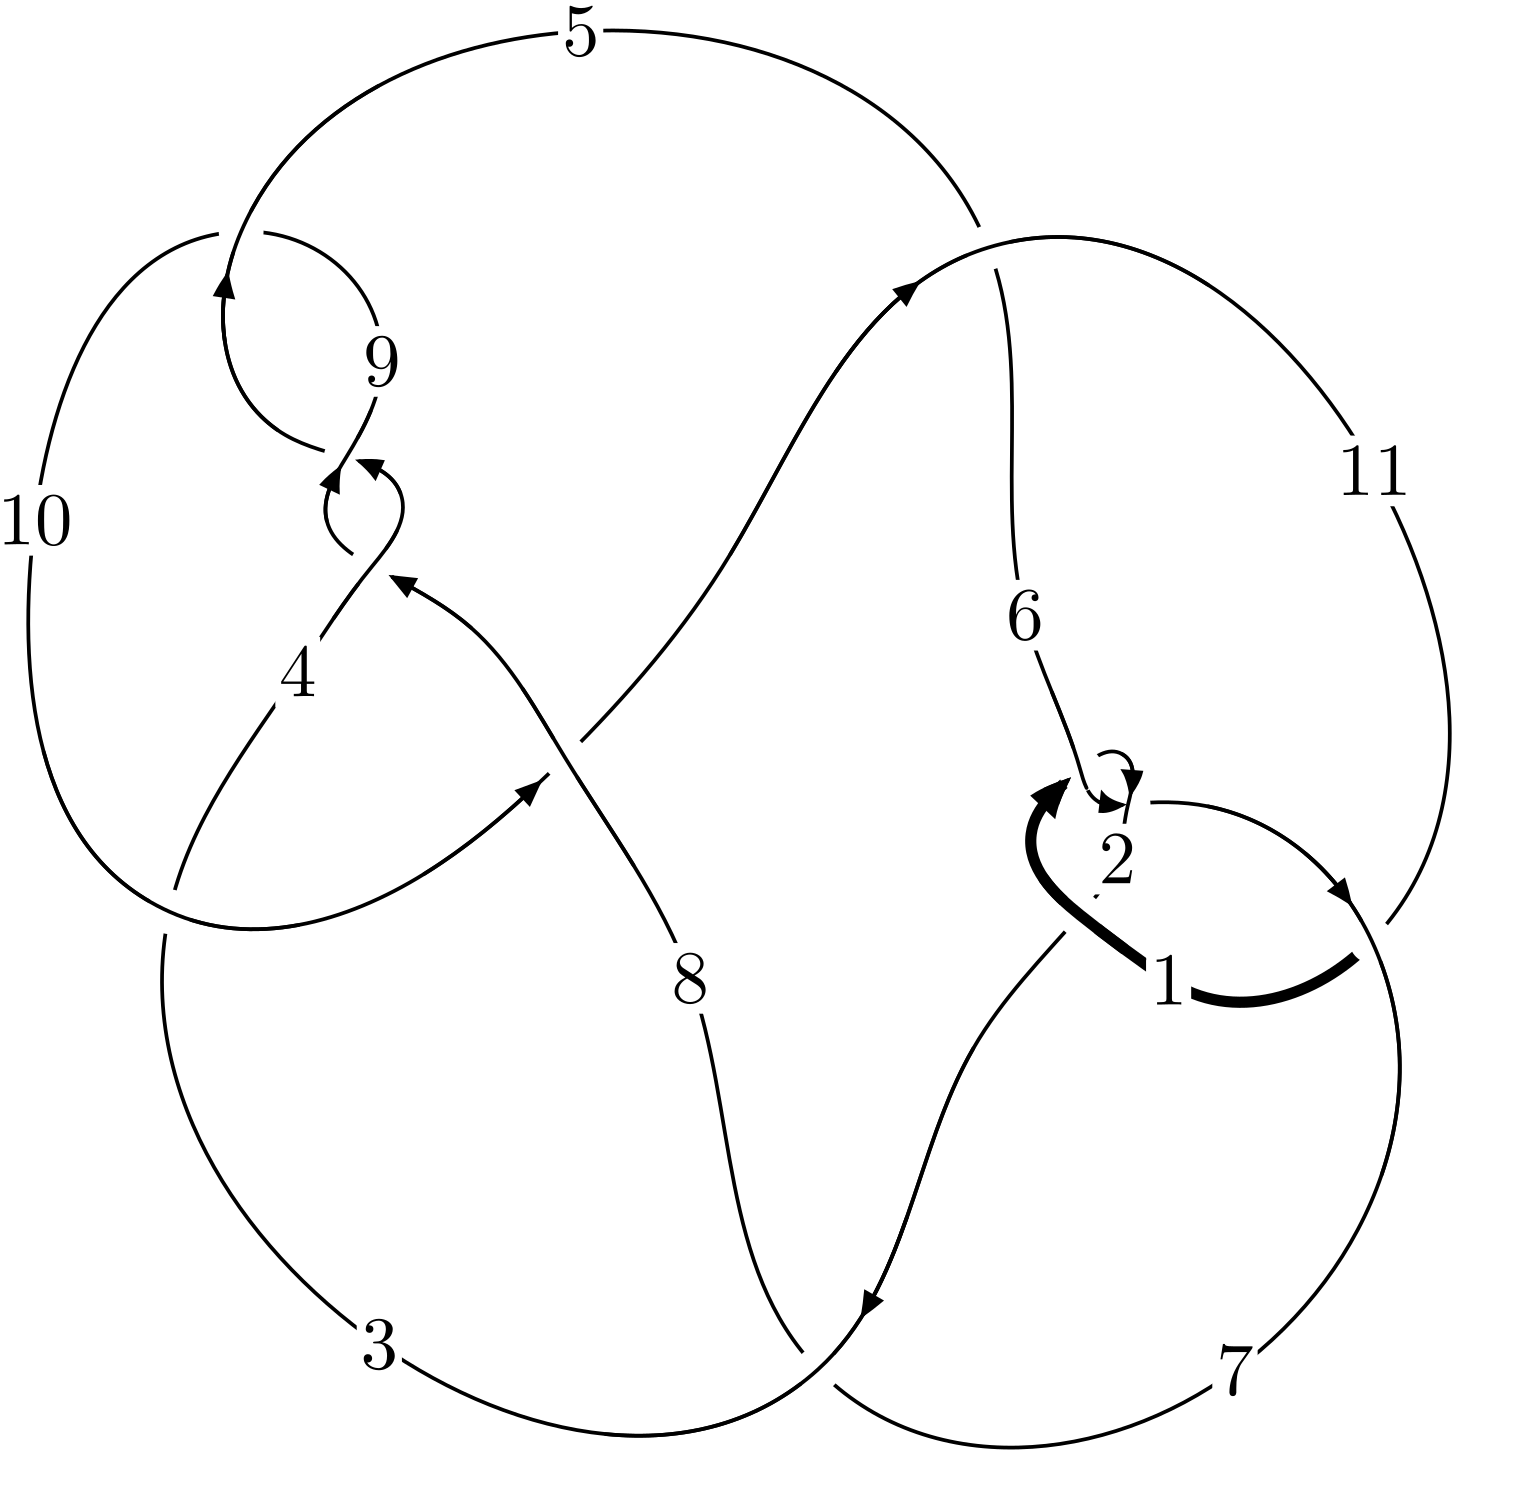
\includegraphics[width=112pt]{../../../GIT/diagram.site/Diagrams/png/425_11a_176.png}\\
\ \ \ A knot diagram\footnotemark}&
\allowdisplaybreaks
\textbf{Linearized knot diagam} \\
\cline{2-2}
 &
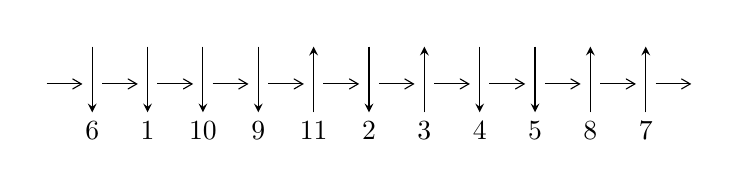
\begin{tikzpicture}[x=20pt, y=17pt]
	% nodes
	\node (C0) at (0, 0) {};
	\node (C1) at (1, 0) {};
	\node (C1U) at (1, +1) {};
	\node (C1D) at (1, -1) {6};

	\node (C2) at (2, 0) {};
	\node (C2U) at (2, +1) {};
	\node (C2D) at (2, -1) {1};

	\node (C3) at (3, 0) {};
	\node (C3U) at (3, +1) {};
	\node (C3D) at (3, -1) {10};

	\node (C4) at (4, 0) {};
	\node (C4U) at (4, +1) {};
	\node (C4D) at (4, -1) {9};

	\node (C5) at (5, 0) {};
	\node (C5U) at (5, +1) {};
	\node (C5D) at (5, -1) {11};

	\node (C6) at (6, 0) {};
	\node (C6U) at (6, +1) {};
	\node (C6D) at (6, -1) {2};

	\node (C7) at (7, 0) {};
	\node (C7U) at (7, +1) {};
	\node (C7D) at (7, -1) {3};

	\node (C8) at (8, 0) {};
	\node (C8U) at (8, +1) {};
	\node (C8D) at (8, -1) {4};

	\node (C9) at (9, 0) {};
	\node (C9U) at (9, +1) {};
	\node (C9D) at (9, -1) {5};

	\node (C10) at (10, 0) {};
	\node (C10U) at (10, +1) {};
	\node (C10D) at (10, -1) {8};

	\node (C11) at (11, 0) {};
	\node (C11U) at (11, +1) {};
	\node (C11D) at (11, -1) {7};
	\node (C12) at (12, 0) {};

	% arrows
	\draw[->,>={angle 60}]
	(C0) edge (C1) (C1) edge (C2) (C2) edge (C3) (C3) edge (C4) (C4) edge (C5) (C5) edge (C6) (C6) edge (C7) (C7) edge (C8) (C8) edge (C9) (C9) edge (C10) (C10) edge (C11) (C11) edge (C12) ;	\draw[->,>=stealth]
	(C1U) edge (C1D) (C2U) edge (C2D) (C3U) edge (C3D) (C4U) edge (C4D) (C5D) edge (C5U) (C6U) edge (C6D) (C7D) edge (C7U) (C8U) edge (C8D) (C9U) edge (C9D) (C10D) edge (C10U) (C11D) edge (C11U) ;
	\end{tikzpicture} \\
\hhline{~~} \\& 
\textbf{Solving Sequence} \\ \cline{2-2} 
 &
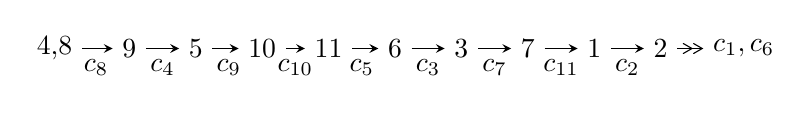
\begin{tikzpicture}[x=24pt, y=7pt]
	% node
	\node (A0) at (-1/8, 0) {4,8};
	\node (A1) at (1, 0) {9};
	\node (A2) at (2, 0) {5};
	\node (A3) at (3, 0) {10};
	\node (A4) at (4, 0) {11};
	\node (A5) at (5, 0) {6};
	\node (A6) at (6, 0) {3};
	\node (A7) at (7, 0) {7};
	\node (A8) at (8, 0) {1};
	\node (A9) at (9, 0) {2};
	\node (C1) at (1/2, -1) {$c_{8}$};
	\node (C2) at (3/2, -1) {$c_{4}$};
	\node (C3) at (5/2, -1) {$c_{9}$};
	\node (C4) at (7/2, -1) {$c_{10}$};
	\node (C5) at (9/2, -1) {$c_{5}$};
	\node (C6) at (11/2, -1) {$c_{3}$};
	\node (C7) at (13/2, -1) {$c_{7}$};
	\node (C8) at (15/2, -1) {$c_{11}$};
	\node (C9) at (17/2, -1) {$c_{2}$};
	\node (A10) at (41/4, 0) {$c_{1},c_{6}$};

	% edge
	\draw[->,>=stealth]	
	(A0) edge (A1) (A1) edge (A2) (A2) edge (A3) (A3) edge (A4) (A4) edge (A5) (A5) edge (A6) (A6) edge (A7) (A7) edge (A8) (A8) edge (A9) ;
	\draw[->>,>={angle 60}]	
	(A9) edge (A10);
\end{tikzpicture} \\ 

\end{tabular} \\

\footnotetext{
The image of knot diagram is generated by the software ``\textbf{Draw programme}" developed by Andrew Bartholomew(\url{http://www.layer8.co.uk/maths/draw/index.htm\#Running-draw}), where we modified some parts for our purpose(\url{https://github.com/CATsTAILs/LinksPainter}).
}\phantom \\ \newline 
\centering \textbf{Ideals for irreducible components\footnotemark of $X_{\text{par}}$} 
 
\begin{align*}
I^u_{1}&=\langle 
u^{54}+2 u^{53}+\cdots- u+1\rangle \\
I^u_{2}&=\langle 
u-1\rangle \\
\\
\end{align*}
\raggedright * 2 irreducible components of $\dim_{\mathbb{C}}=0$, with total 55 representations.\\
\footnotetext{All coefficients of polynomials are rational numbers. But the coefficients are sometimes approximated in decimal forms when there is not enough margin.}
\newpage
\renewcommand{\arraystretch}{1}
\centering \section*{I. $I^u_{1}= \langle u^{54}+2 u^{53}+\cdots- u+1 \rangle$}
\flushleft \textbf{(i) Arc colorings}\\
\begin{tabular}{m{7pt} m{180pt} m{7pt} m{180pt} }
\flushright $a_{4}=$&$\begin{pmatrix}0\\u\end{pmatrix}$ \\
\flushright $a_{8}=$&$\begin{pmatrix}1\\0\end{pmatrix}$ \\
\flushright $a_{9}=$&$\begin{pmatrix}1\\u^2\end{pmatrix}$ \\
\flushright $a_{5}=$&$\begin{pmatrix}- u\\- u^3+u\end{pmatrix}$ \\
\flushright $a_{10}=$&$\begin{pmatrix}- u^2+1\\- u^4+2 u^2\end{pmatrix}$ \\
\flushright $a_{11}=$&$\begin{pmatrix}- u^4+u^2+1\\- u^4+2 u^2\end{pmatrix}$ \\
\flushright $a_{6}=$&$\begin{pmatrix}- u^{11}+4 u^9-4 u^7-2 u^5+3 u^3\\- u^{11}+5 u^9-8 u^7+3 u^5+u^3+u\end{pmatrix}$ \\
\flushright $a_{3}=$&$\begin{pmatrix}u^5-2 u^3+u\\u^7-3 u^5+2 u^3+u\end{pmatrix}$ \\
\flushright $a_{7}=$&$\begin{pmatrix}u^{12}-5 u^{10}+9 u^8-6 u^6+u^2+1\\u^{14}-6 u^{12}+13 u^{10}-10 u^8-2 u^6+4 u^4+u^2\end{pmatrix}$ \\
\flushright $a_{1}=$&$\begin{pmatrix}u^{30}-13 u^{28}+\cdots+2 u^2+1\\u^{32}-14 u^{30}+\cdots-20 u^8+2 u^2\end{pmatrix}$ \\
\flushright $a_{2}=$&$\begin{pmatrix}2 u^{53}+u^{52}+\cdots- u+2\\2 u^{53}+2 u^{52}+\cdots- u+1\end{pmatrix}$\\ \flushright $a_{2}=$&$\begin{pmatrix}2 u^{53}+u^{52}+\cdots- u+2\\2 u^{53}+2 u^{52}+\cdots- u+1\end{pmatrix}$\\&\end{tabular}
\flushleft \textbf{(ii) Obstruction class $= -1$}\\~\\
\flushleft \textbf{(iii) Cusp Shapes $= -4 u^{53}+96 u^{51}+\cdots+12 u-10$}\\~\\
\newpage\renewcommand{\arraystretch}{1}
\flushleft \textbf{(iv) u-Polynomials at the component}\newline \\
\begin{tabular}{m{50pt}|m{274pt}}
Crossings & \hspace{64pt}u-Polynomials at each crossing \\
\hline $$\begin{aligned}c_{1},c_{6}\end{aligned}$$&$\begin{aligned}
&u^{54}-2 u^{53}+\cdots- u+1
\end{aligned}$\\
\hline $$\begin{aligned}c_{2}\end{aligned}$$&$\begin{aligned}
&u^{54}+24 u^{53}+\cdots- u+1
\end{aligned}$\\
\hline $$\begin{aligned}c_{3}\end{aligned}$$&$\begin{aligned}
&u^{54}+3 u^{53}+\cdots+13 u+5
\end{aligned}$\\
\hline $$\begin{aligned}c_{4},c_{8},c_{9}\end{aligned}$$&$\begin{aligned}
&u^{54}-2 u^{53}+\cdots+u+1
\end{aligned}$\\
\hline $$\begin{aligned}c_{5},c_{7}\end{aligned}$$&$\begin{aligned}
&u^{54}-20 u^{52}+\cdots-23 u+1
\end{aligned}$\\
\hline $$\begin{aligned}c_{10}\end{aligned}$$&$\begin{aligned}
&u^{54}+12 u^{53}+\cdots+297 u+23
\end{aligned}$\\
\hline $$\begin{aligned}c_{11}\end{aligned}$$&$\begin{aligned}
&u^{54}-3 u^{53}+\cdots+11 u+5
\end{aligned}$\\
\hline
\end{tabular}\\~\\
\newpage\renewcommand{\arraystretch}{1}
\flushleft \textbf{(v) Riley Polynomials at the component}\newline \\
\begin{tabular}{m{50pt}|m{274pt}}
Crossings & \hspace{64pt}Riley Polynomials at each crossing \\
\hline $$\begin{aligned}c_{1},c_{6}\end{aligned}$$&$\begin{aligned}
&y^{54}-24 y^{53}+\cdots+y+1
\end{aligned}$\\
\hline $$\begin{aligned}c_{2}\end{aligned}$$&$\begin{aligned}
&y^{54}+12 y^{53}+\cdots-11 y+1
\end{aligned}$\\
\hline $$\begin{aligned}c_{3}\end{aligned}$$&$\begin{aligned}
&y^{54}+3 y^{53}+\cdots-269 y+25
\end{aligned}$\\
\hline $$\begin{aligned}c_{4},c_{8},c_{9}\end{aligned}$$&$\begin{aligned}
&y^{54}-48 y^{53}+\cdots+y+1
\end{aligned}$\\
\hline $$\begin{aligned}c_{5},c_{7}\end{aligned}$$&$\begin{aligned}
&y^{54}-40 y^{53}+\cdots-207 y+1
\end{aligned}$\\
\hline $$\begin{aligned}c_{10}\end{aligned}$$&$\begin{aligned}
&y^{54}+8 y^{53}+\cdots+11749 y+529
\end{aligned}$\\
\hline $$\begin{aligned}c_{11}\end{aligned}$$&$\begin{aligned}
&y^{54}+3 y^{53}+\cdots+1139 y+25
\end{aligned}$\\
\hline
\end{tabular}\\~\\
\newpage\flushleft \textbf{(vi) Complex Volumes and Cusp Shapes}
$$\begin{array}{c|c|c}  
\text{Solutions to }I^u_{1}& \I (\text{vol} + \sqrt{-1}CS) & \text{Cusp shape}\\
 \hline 
\begin{aligned}
u &= \phantom{-}0.963853 + 0.239721 I\end{aligned}
 & \phantom{-}1.70219 - 6.38060 I & -2.45012 + 6.07310 I \\ \hline\begin{aligned}
u &= \phantom{-}0.963853 - 0.239721 I\end{aligned}
 & \phantom{-}1.70219 + 6.38060 I & -2.45012 - 6.07310 I \\ \hline\begin{aligned}
u &= -0.915784 + 0.228115 I\end{aligned}
 & \phantom{-}3.41733 + 1.25909 I & \phantom{-}0.259004 - 1.112987 I \\ \hline\begin{aligned}
u &= -0.915784 - 0.228115 I\end{aligned}
 & \phantom{-}3.41733 - 1.25909 I & \phantom{-}0.259004 + 1.112987 I \\ \hline\begin{aligned}
u &= -0.789465 + 0.267366 I\end{aligned}
 & \phantom{-}3.26830 - 1.40826 I & -0.268768 - 0.442670 I \\ \hline\begin{aligned}
u &= -0.789465 - 0.267366 I\end{aligned}
 & \phantom{-}3.26830 + 1.40826 I & -0.268768 + 0.442670 I \\ \hline\begin{aligned}
u &= \phantom{-}0.758491 + 0.308061 I\end{aligned}
 & \phantom{-}1.40844 + 6.51845 I & -3.38857 - 4.08750 I \\ \hline\begin{aligned}
u &= \phantom{-}0.758491 - 0.308061 I\end{aligned}
 & \phantom{-}1.40844 - 6.51845 I & -3.38857 + 4.08750 I \\ \hline\begin{aligned}
u &= \phantom{-}0.256667 + 0.732348 I\end{aligned}
 & \phantom{-}3.15875 - 10.41640 I & -0.77334 + 8.79469 I \\ \hline\begin{aligned}
u &= \phantom{-}0.256667 - 0.732348 I\end{aligned}
 & \phantom{-}3.15875 + 10.41640 I & -0.77334 - 8.79469 I \\ \hline\begin{aligned}
u &= -0.243755 + 0.728305 I\end{aligned}
 & \phantom{-}5.12841 + 5.22917 I & \phantom{-}2.37428 - 4.44764 I \\ \hline\begin{aligned}
u &= -0.243755 - 0.728305 I\end{aligned}
 & \phantom{-}5.12841 - 5.22917 I & \phantom{-}2.37428 + 4.44764 I \\ \hline\begin{aligned}
u &= -0.206060 + 0.723757 I\end{aligned}
 & \phantom{-}5.62286 + 2.45822 I & \phantom{-}3.43259 - 3.89075 I \\ \hline\begin{aligned}
u &= -0.206060 - 0.723757 I\end{aligned}
 & \phantom{-}5.62286 - 2.45822 I & \phantom{-}3.43259 + 3.89075 I \\ \hline\begin{aligned}
u &= \phantom{-}0.185877 + 0.724088 I\end{aligned}
 & \phantom{-}4.07878 + 2.66694 I & \phantom{-}1.14279 - 1.40015 I \\ \hline\begin{aligned}
u &= \phantom{-}0.185877 - 0.724088 I\end{aligned}
 & \phantom{-}4.07878 - 2.66694 I & \phantom{-}1.14279 + 1.40015 I \\ \hline\begin{aligned}
u &= \phantom{-}0.248073 + 0.690816 I\end{aligned}
 & \phantom{-}0.11288 - 3.24680 I & -3.97449 + 4.31964 I \\ \hline\begin{aligned}
u &= \phantom{-}0.248073 - 0.690816 I\end{aligned}
 & \phantom{-}0.11288 + 3.24680 I & -3.97449 - 4.31964 I \\ \hline\begin{aligned}
u &= \phantom{-}1.275390 + 0.130366 I\end{aligned}
 & -2.32233 - 0.58829 I & \phantom{-0.000000 } 0 \\ \hline\begin{aligned}
u &= \phantom{-}1.275390 - 0.130366 I\end{aligned}
 & -2.32233 + 0.58829 I & \phantom{-0.000000 } 0 \\ \hline\begin{aligned}
u &= -1.301090 + 0.201573 I\end{aligned}
 & -3.00640 + 4.83893 I & \phantom{-0.000000 } 0 \\ \hline\begin{aligned}
u &= -1.301090 - 0.201573 I\end{aligned}
 & -3.00640 - 4.83893 I & \phantom{-0.000000 } 0 \\ \hline\begin{aligned}
u &= -0.335824 + 0.569569 I\end{aligned}
 & -2.75425 + 5.16303 I & -6.62576 - 8.31738 I \\ \hline\begin{aligned}
u &= -0.335824 - 0.569569 I\end{aligned}
 & -2.75425 - 5.16303 I & -6.62576 + 8.31738 I \\ \hline\begin{aligned}
u &= -0.388647 + 0.474801 I\end{aligned}
 & -3.08098 - 1.83888 I & -8.29710 + 0.16550 I \\ \hline\begin{aligned}
u &= -0.388647 - 0.474801 I\end{aligned}
 & -3.08098 + 1.83888 I & -8.29710 - 0.16550 I \\ \hline\begin{aligned}
u &= \phantom{-}1.389140 + 0.067526 I\end{aligned}
 & -3.09355 + 0.76124 I & \phantom{-0.000000 } 0 \\ \hline\begin{aligned}
u &= \phantom{-}1.389140 - 0.067526 I\end{aligned}
 & -3.09355 - 0.76124 I & \phantom{-0.000000 } 0 \\ \hline\begin{aligned}
u &= -1.367000 + 0.288368 I\end{aligned}
 & -0.833592 + 0.995204 I & \phantom{-0.000000 } 0 \\ \hline\begin{aligned}
u &= -1.367000 - 0.288368 I\end{aligned}
 & -0.833592 - 0.995204 I & \phantom{-0.000000 } 0\\
 \hline 
 \end{array}$$\newpage$$\begin{array}{c|c|c}  
\text{Solutions to }I^u_{1}& \I (\text{vol} + \sqrt{-1}CS) & \text{Cusp shape}\\
 \hline 
\begin{aligned}
u &= \phantom{-}0.059975 + 0.594195 I\end{aligned}
 & \phantom{-}1.20313 - 1.95407 I & \phantom{-}2.79385 + 4.45291 I \\ \hline\begin{aligned}
u &= \phantom{-}0.059975 - 0.594195 I\end{aligned}
 & \phantom{-}1.20313 + 1.95407 I & \phantom{-}2.79385 - 4.45291 I \\ \hline\begin{aligned}
u &= -1.400510 + 0.118575 I\end{aligned}
 & -7.31911 + 1.48659 I & \phantom{-0.000000 } 0 \\ \hline\begin{aligned}
u &= -1.400510 - 0.118575 I\end{aligned}
 & -7.31911 - 1.48659 I & \phantom{-0.000000 } 0 \\ \hline\begin{aligned}
u &= \phantom{-}1.378690 + 0.289179 I\end{aligned}
 & \phantom{-}0.59736 - 6.12710 I & \phantom{-0.000000 } 0 \\ \hline\begin{aligned}
u &= \phantom{-}1.378690 - 0.289179 I\end{aligned}
 & \phantom{-}0.59736 + 6.12710 I & \phantom{-0.000000 } 0 \\ \hline\begin{aligned}
u &= -1.396360 + 0.208440 I\end{aligned}
 & -5.56771 + 4.07219 I & \phantom{-0.000000 } 0 \\ \hline\begin{aligned}
u &= -1.396360 - 0.208440 I\end{aligned}
 & -5.56771 - 4.07219 I & \phantom{-0.000000 } 0 \\ \hline\begin{aligned}
u &= -1.41551 + 0.07207 I\end{aligned}
 & -5.12761 - 5.61169 I & \phantom{-0.000000 } 0 \\ \hline\begin{aligned}
u &= -1.41551 - 0.07207 I\end{aligned}
 & -5.12761 + 5.61169 I & \phantom{-0.000000 } 0 \\ \hline\begin{aligned}
u &= \phantom{-}0.544247 + 0.205329 I\end{aligned}
 & -1.48527 - 0.15164 I & -7.75648 + 0.91671 I \\ \hline\begin{aligned}
u &= \phantom{-}0.544247 - 0.205329 I\end{aligned}
 & -1.48527 + 0.15164 I & -7.75648 - 0.91671 I \\ \hline\begin{aligned}
u &= \phantom{-}0.274528 + 0.511538 I\end{aligned}
 & -0.243608 - 1.371010 I & -2.52596 + 5.06044 I \\ \hline\begin{aligned}
u &= \phantom{-}0.274528 - 0.511538 I\end{aligned}
 & -0.243608 + 1.371010 I & -2.52596 - 5.06044 I \\ \hline\begin{aligned}
u &= -1.39901 + 0.27445 I\end{aligned}
 & -5.13575 + 6.76281 I & \phantom{-0.000000 } 0 \\ \hline\begin{aligned}
u &= -1.39901 - 0.27445 I\end{aligned}
 & -5.13575 - 6.76281 I & \phantom{-0.000000 } 0 \\ \hline\begin{aligned}
u &= \phantom{-}1.41497 + 0.18855 I\end{aligned}
 & -8.77151 - 0.63321 I & \phantom{-0.000000 } 0 \\ \hline\begin{aligned}
u &= \phantom{-}1.41497 - 0.18855 I\end{aligned}
 & -8.77151 + 0.63321 I & \phantom{-0.000000 } 0 \\ \hline\begin{aligned}
u &= \phantom{-}1.39845 + 0.29073 I\end{aligned}
 & -0.09729 - 8.92706 I & \phantom{-0.000000 } 0 \\ \hline\begin{aligned}
u &= \phantom{-}1.39845 - 0.29073 I\end{aligned}
 & -0.09729 + 8.92706 I & \phantom{-0.000000 } 0 \\ \hline\begin{aligned}
u &= \phantom{-}1.41558 + 0.21956 I\end{aligned}
 & -8.33472 - 8.06621 I & \phantom{-0.000000 } 0 \\ \hline\begin{aligned}
u &= \phantom{-}1.41558 - 0.21956 I\end{aligned}
 & -8.33472 + 8.06621 I & \phantom{-0.000000 } 0 \\ \hline\begin{aligned}
u &= -1.40491 + 0.29196 I\end{aligned}
 & -2.1336 + 14.1348 I & \phantom{-0.000000 } 0 \\ \hline\begin{aligned}
u &= -1.40491 - 0.29196 I\end{aligned}
 & -2.1336 - 14.1348 I & \phantom{-0.000000 } 0\\
 \hline 
 \end{array}$$\newpage\newpage\renewcommand{\arraystretch}{1}
\centering \section*{II. $I^u_{2}= \langle u-1 \rangle$}
\flushleft \textbf{(i) Arc colorings}\\
\begin{tabular}{m{7pt} m{180pt} m{7pt} m{180pt} }
\flushright $a_{4}=$&$\begin{pmatrix}0\\1\end{pmatrix}$ \\
\flushright $a_{8}=$&$\begin{pmatrix}1\\0\end{pmatrix}$ \\
\flushright $a_{9}=$&$\begin{pmatrix}1\\1\end{pmatrix}$ \\
\flushright $a_{5}=$&$\begin{pmatrix}-1\\0\end{pmatrix}$ \\
\flushright $a_{10}=$&$\begin{pmatrix}0\\1\end{pmatrix}$ \\
\flushright $a_{11}=$&$\begin{pmatrix}1\\1\end{pmatrix}$ \\
\flushright $a_{6}=$&$\begin{pmatrix}0\\1\end{pmatrix}$ \\
\flushright $a_{3}=$&$\begin{pmatrix}0\\1\end{pmatrix}$ \\
\flushright $a_{7}=$&$\begin{pmatrix}1\\1\end{pmatrix}$ \\
\flushright $a_{1}=$&$\begin{pmatrix}1\\1\end{pmatrix}$ \\
\flushright $a_{2}=$&$\begin{pmatrix}1\\2\end{pmatrix}$\\ \flushright $a_{2}=$&$\begin{pmatrix}1\\2\end{pmatrix}$\\&\end{tabular}
\flushleft \textbf{(ii) Obstruction class $= -1$}\\~\\
\flushleft \textbf{(iii) Cusp Shapes $= -6$}\\~\\
\newpage\renewcommand{\arraystretch}{1}
\flushleft \textbf{(iv) u-Polynomials at the component}\newline \\
\begin{tabular}{m{50pt}|m{274pt}}
Crossings & \hspace{64pt}u-Polynomials at each crossing \\
\hline $$\begin{aligned}c_{1},c_{2},c_{4}\\c_{5},c_{6},c_{7}\\c_{8},c_{9},c_{10}\end{aligned}$$&$\begin{aligned}
&u+1
\end{aligned}$\\
\hline $$\begin{aligned}c_{3},c_{11}\end{aligned}$$&$\begin{aligned}
&u
\end{aligned}$\\
\hline
\end{tabular}\\~\\
\newpage\renewcommand{\arraystretch}{1}
\flushleft \textbf{(v) Riley Polynomials at the component}\newline \\
\begin{tabular}{m{50pt}|m{274pt}}
Crossings & \hspace{64pt}Riley Polynomials at each crossing \\
\hline $$\begin{aligned}c_{1},c_{2},c_{4}\\c_{5},c_{6},c_{7}\\c_{8},c_{9},c_{10}\end{aligned}$$&$\begin{aligned}
&y-1
\end{aligned}$\\
\hline $$\begin{aligned}c_{3},c_{11}\end{aligned}$$&$\begin{aligned}
&y
\end{aligned}$\\
\hline
\end{tabular}\\~\\
\newpage\flushleft \textbf{(vi) Complex Volumes and Cusp Shapes}
$$\begin{array}{c|c|c}  
\text{Solutions to }I^u_{2}& \I (\text{vol} + \sqrt{-1}CS) & \text{Cusp shape}\\
 \hline 
\begin{aligned}
u &= \phantom{-}1.00000\phantom{ +0.000000I}\end{aligned}
 & -1.64493\phantom{ +0.000000I} & -6.00000\phantom{ +0.000000I}\\
 \hline 
 \end{array}$$\newpage
\newpage\renewcommand{\arraystretch}{1}
\centering \section*{ III. u-Polynomials}
\begin{tabular}{m{50pt}|m{274pt}}
Crossings & \hspace{64pt}u-Polynomials at each crossing \\
\hline $$\begin{aligned}c_{1},c_{6}\end{aligned}$$&$\begin{aligned}
&(u+1)(u^{54}-2 u^{53}+\cdots- u+1)
\end{aligned}$\\
\hline $$\begin{aligned}c_{2}\end{aligned}$$&$\begin{aligned}
&(u+1)(u^{54}+24 u^{53}+\cdots- u+1)
\end{aligned}$\\
\hline $$\begin{aligned}c_{3}\end{aligned}$$&$\begin{aligned}
&u(u^{54}+3 u^{53}+\cdots+13 u+5)
\end{aligned}$\\
\hline $$\begin{aligned}c_{4},c_{8},c_{9}\end{aligned}$$&$\begin{aligned}
&(u+1)(u^{54}-2 u^{53}+\cdots+u+1)
\end{aligned}$\\
\hline $$\begin{aligned}c_{5},c_{7}\end{aligned}$$&$\begin{aligned}
&(u+1)(u^{54}-20 u^{52}+\cdots-23 u+1)
\end{aligned}$\\
\hline $$\begin{aligned}c_{10}\end{aligned}$$&$\begin{aligned}
&(u+1)(u^{54}+12 u^{53}+\cdots+297 u+23)
\end{aligned}$\\
\hline $$\begin{aligned}c_{11}\end{aligned}$$&$\begin{aligned}
&u(u^{54}-3 u^{53}+\cdots+11 u+5)
\end{aligned}$\\
\hline
\end{tabular}\newpage\renewcommand{\arraystretch}{1}
\centering \section*{ IV. Riley Polynomials}
\begin{tabular}{m{50pt}|m{274pt}}
Crossings & \hspace{64pt}Riley Polynomials at each crossing \\
\hline $$\begin{aligned}c_{1},c_{6}\end{aligned}$$&$\begin{aligned}
&(y-1)(y^{54}-24 y^{53}+\cdots+y+1)
\end{aligned}$\\
\hline $$\begin{aligned}c_{2}\end{aligned}$$&$\begin{aligned}
&(y-1)(y^{54}+12 y^{53}+\cdots-11 y+1)
\end{aligned}$\\
\hline $$\begin{aligned}c_{3}\end{aligned}$$&$\begin{aligned}
&y(y^{54}+3 y^{53}+\cdots-269 y+25)
\end{aligned}$\\
\hline $$\begin{aligned}c_{4},c_{8},c_{9}\end{aligned}$$&$\begin{aligned}
&(y-1)(y^{54}-48 y^{53}+\cdots+y+1)
\end{aligned}$\\
\hline $$\begin{aligned}c_{5},c_{7}\end{aligned}$$&$\begin{aligned}
&(y-1)(y^{54}-40 y^{53}+\cdots-207 y+1)
\end{aligned}$\\
\hline $$\begin{aligned}c_{10}\end{aligned}$$&$\begin{aligned}
&(y-1)(y^{54}+8 y^{53}+\cdots+11749 y+529)
\end{aligned}$\\
\hline $$\begin{aligned}c_{11}\end{aligned}$$&$\begin{aligned}
&y(y^{54}+3 y^{53}+\cdots+1139 y+25)
\end{aligned}$\\
\hline
\end{tabular}
\vskip 2pc
\end{document}